%------------------------------------------------------------------------
%Editar Diplomado
\hypertarget{cv:modificarMensaje}{\section{Modificar Mensaje}} \label{sec:modificarMensaje}

	Esta funcionalidad le permitirá modificar la información de un mensaje previamente registrado con el fin de corregir o actualizar datos del mismo. 

		\subsection{Procedimiento}

			%Pasos de procedimiento
			\begin{enumerate}
	
			\item Oprima el botón \IUEditar{} de algún registro existente de la pantalla \ref{fig:GestionarMensajes} ''Gestionar Mensajes''.
	
			\item Se mostrará la pantalla \ref{fig:modificarMensaje} ''Modificar Mensaje''.
			
			%Pantalla
			\begin{figure}[H]
				\begin{center}
					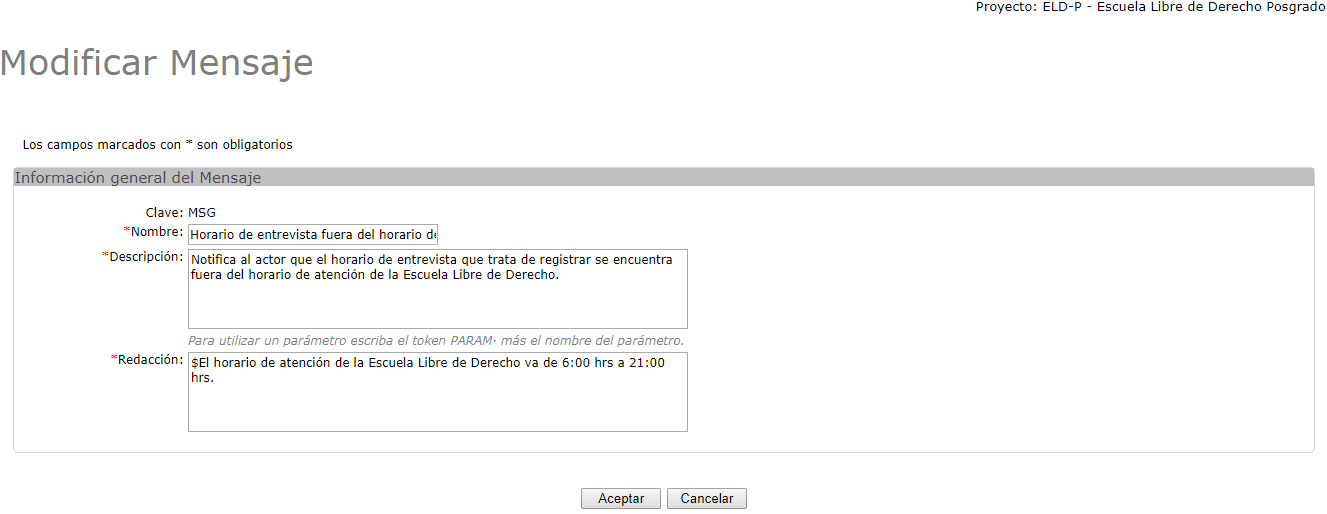
\includegraphics[scale=0.5]{roles/lider/mensajes/pantallas/IU9-2modificarMensaje}
					\caption{Modificar Mensaje}
					\label{fig:modificarMensaje}
				\end{center}
			\end{figure}
		
			
			\item Si el mensaje tiene parámetros se mostrará la pantalla de la siguiente manera.
			
			\begin{figure}[H]
				\begin{center}
					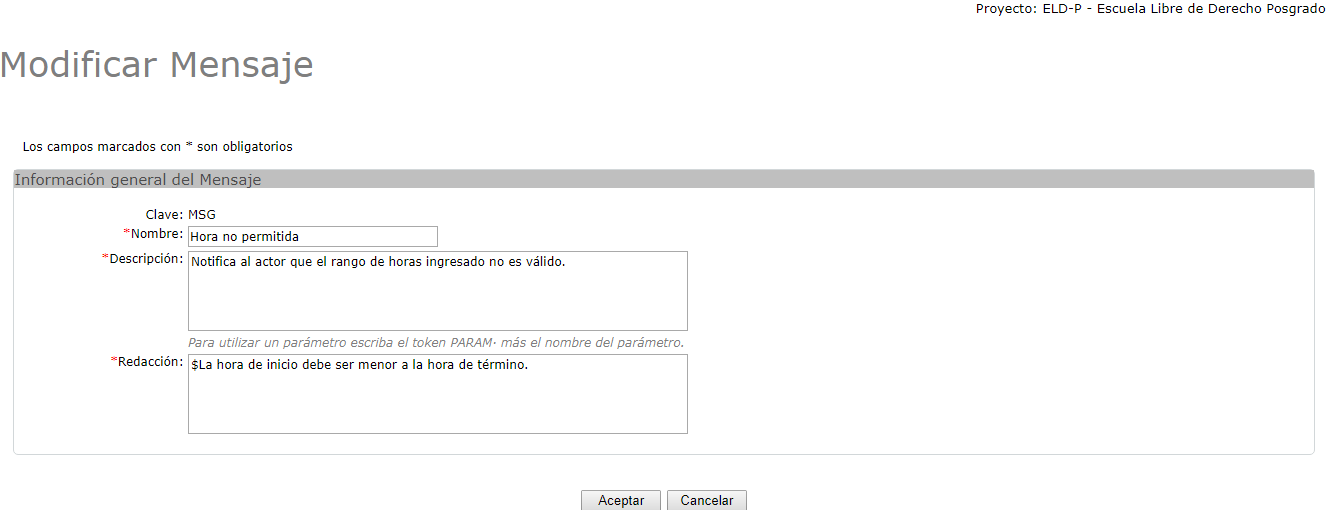
\includegraphics[scale=0.5]{roles/lider/mensajes/pantallas/IU9-2modificarMensajeParam}
					\caption{Modificar Mensaje Parametrizado}
					\label{fig:modificarMensajeParam}
				\end{center}
			\end{figure}
		
			\item Modifique los datos solicitados por la pantalla.
						
			\item Oprima el botón \IUAceptar.
			
			\item Se mostrará el mensaje \ref{fig:mensajeModificado} en la pantalla \ref{fig:GestionarMensajes} ''Gestionar Mensajes''.
			
			\begin{figure}[htbp!]
				\begin{center}
					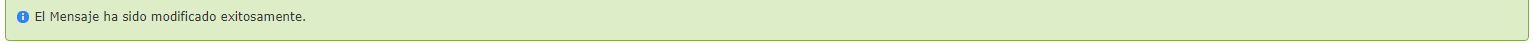
\includegraphics[scale=0.40]{roles/lider/mensajes/pantallas/IU9-2MSG1}
					\caption{MSG: Mensaje Actualizado}
					\label{fig:mensajeModificado}
				\end{center}
			\end{figure}
			\end{enumerate}